\documentclass{standalone}
\usepackage{tikz}

\begin{document}


\begin{tikzpicture}[step=.5cm]


\begin{scope}[scale=3]
%\clip (0,0) circle (10mm);
\path (0,-2pt) node {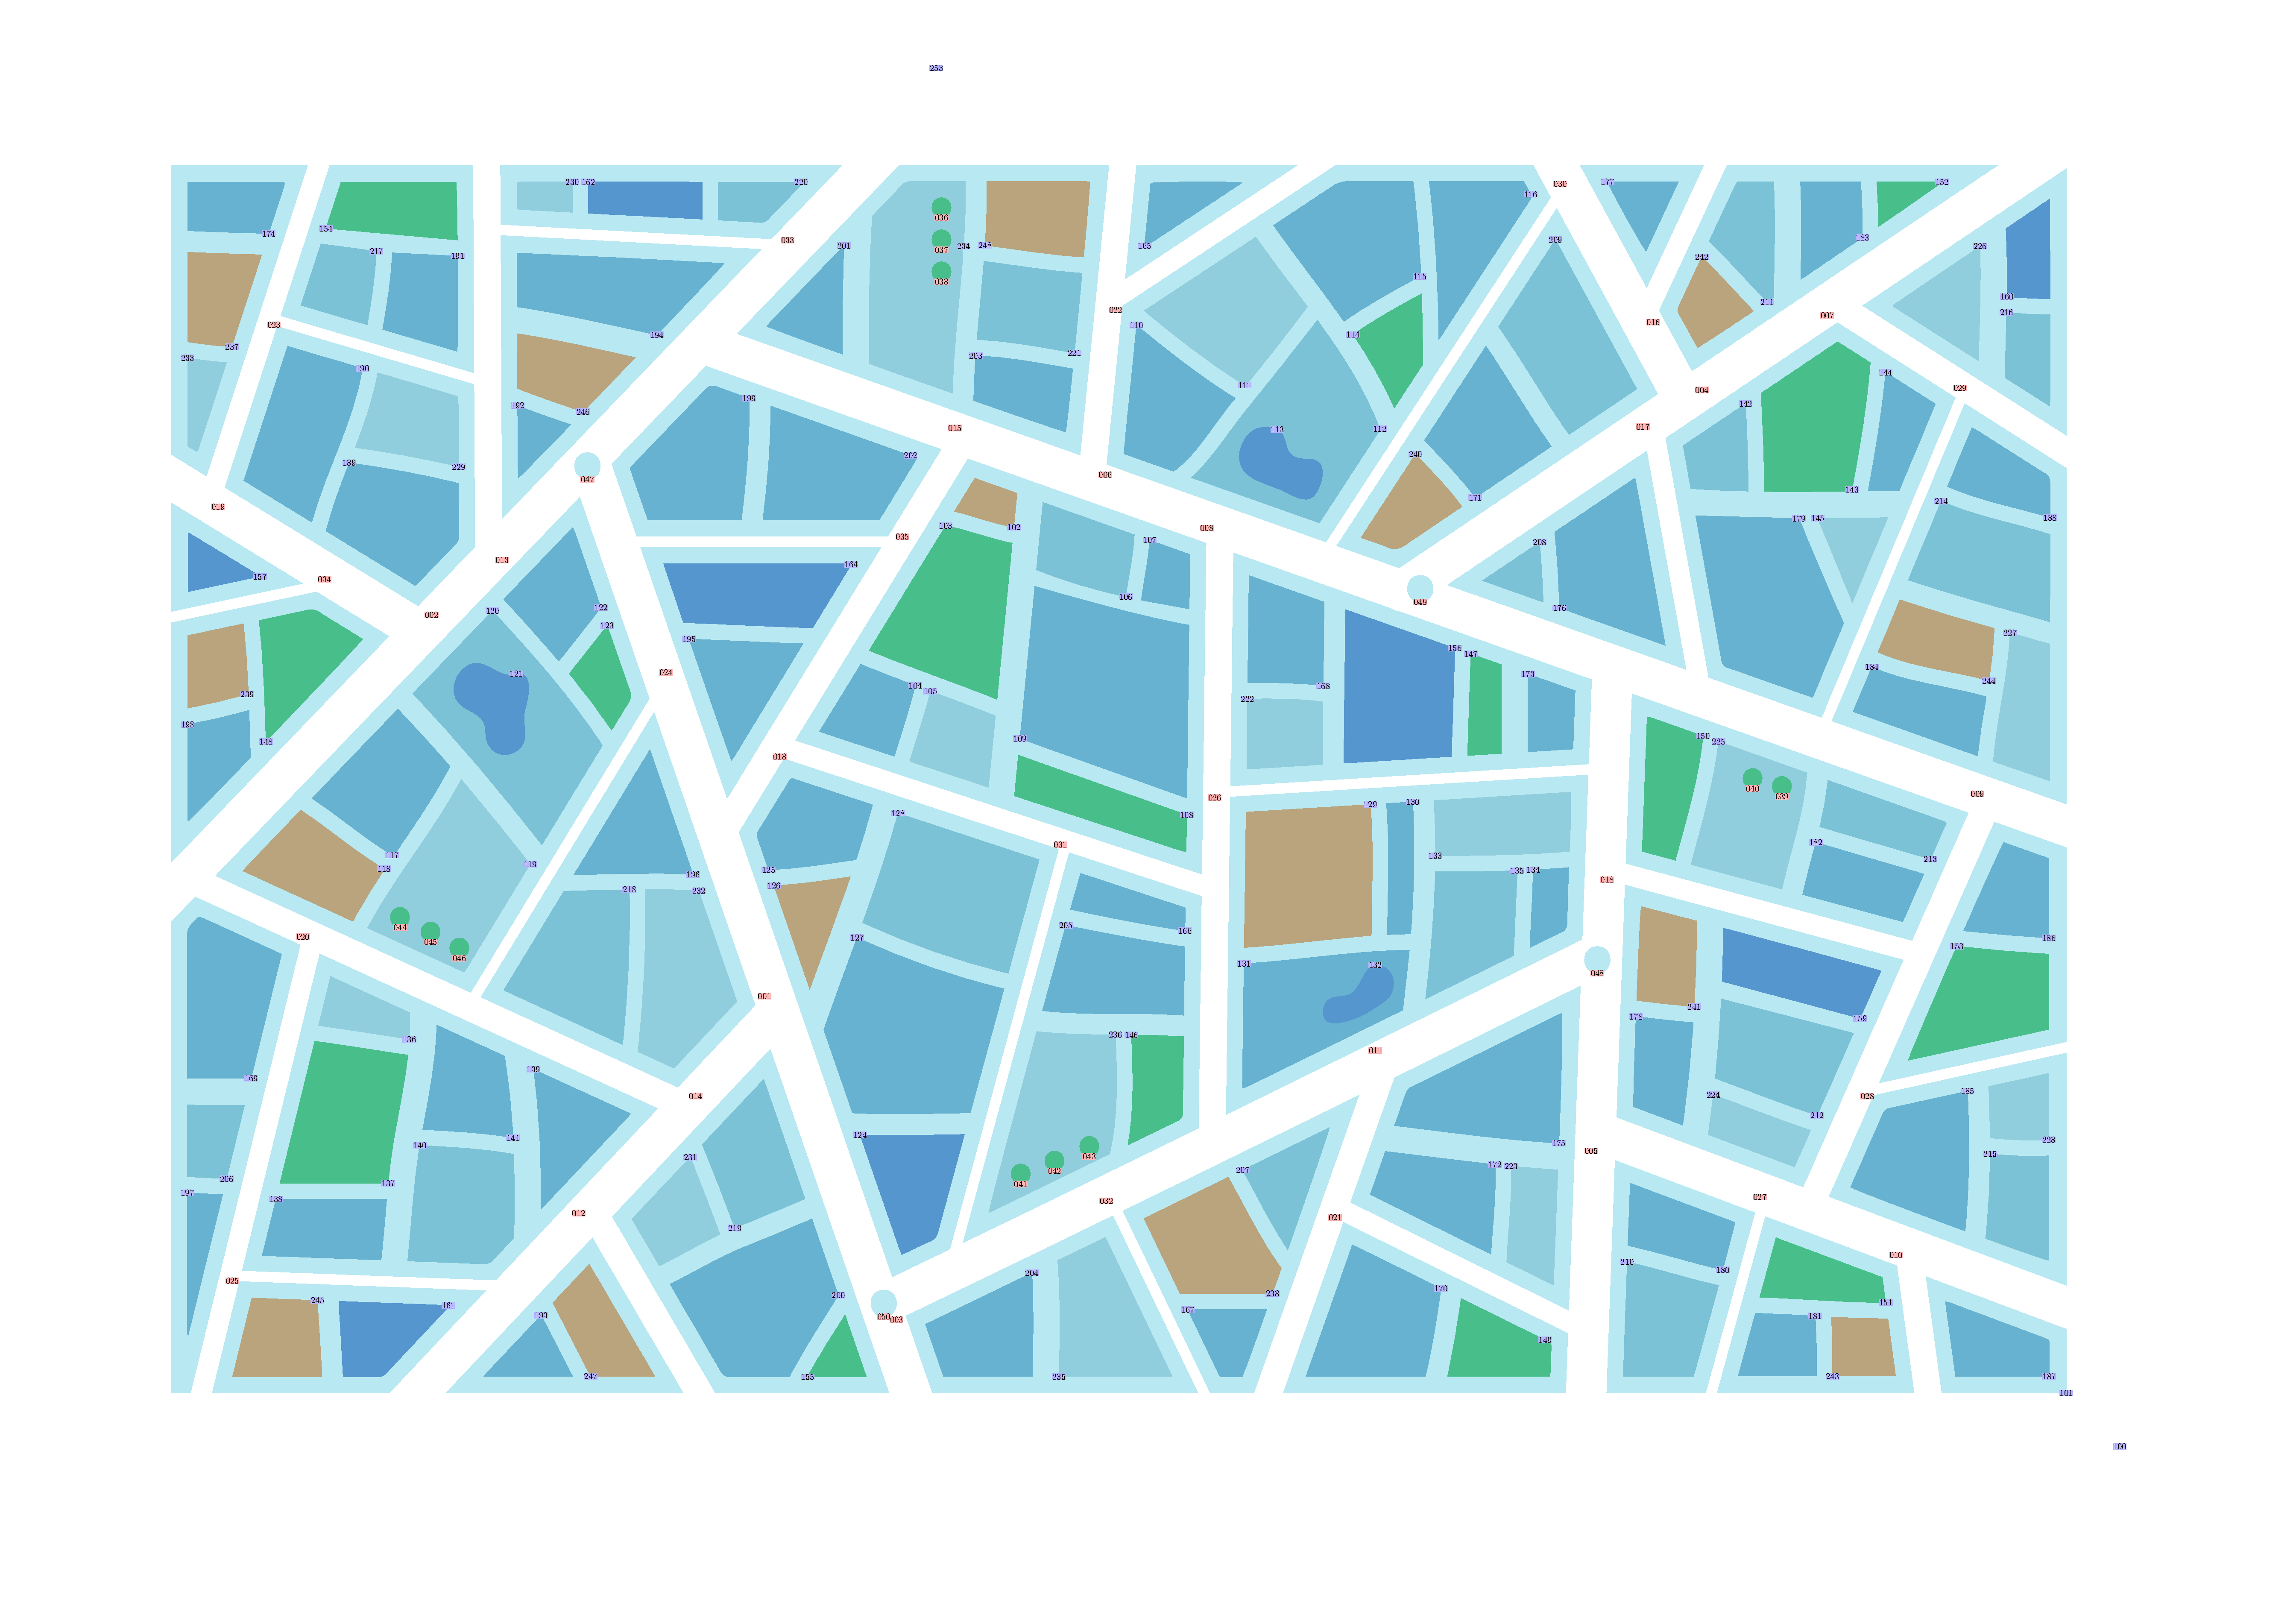
\includegraphics[width=\textwidth]{map2.pdf}};
\end{scope}

%\draw[help lines,black!30,step=.5] (-5.5,-3.5) grid (5.5,3.5);
%\draw[->] (0,-5) -- (0,5) node[left]  {y};\draw[thick,->] (-5,0) -- (5,0) node[below] {x};
%\foreach \x in {-4,-3,-2,-1,1,2,3,4} \node[left] at (0,\x) {\tiny\x} node[below] at (\x,0) {\tiny\x};\node[below right,color=red!20] at (0,0) {\tiny 0}; 

\end{tikzpicture}
\end{document}